\documentclass[a4paper, 12pt]{extreport}
\usepackage[margin=1in]{geometry}
\usepackage{parskip}
\setlength{\parindent}{1cm}
\setlength{\parskip}{.5\baselineskip}
\usepackage{tikz}
\usepackage{setspace}
\graphicspath{ {../../resources/images/} }
\usepackage[titles]{tocloft}
\usepackage{titlesec}
\usepackage[hidelinks]{hyperref}
\usepackage{pdfpages}
\titleformat{\chapter}[hang]{\huge\bfseries}{\thechapter}{20pt}{\vspace{0.5em}}
\titlespacing*{\chapter}{0pt}{-3em}{1.1\parskip}
\usepackage[backend=biber, style=ieee]{biblatex}
\usepackage[nottoc,numbib]{tocbibind}
\usepackage{pgfgantt}
\renewbibmacro{finentry}{\finentry%
	\iffieldundef{annotation}
	{}
	{\par\medskip\printfield{annotation}\medskip\finentry}}

\addbibresource{../../resources/citation.bib}

\begin{document}
	
	\onehalfspacing
	
	\begin{titlepage}
		
		\begin{tikzpicture}[remember picture, overlay]
			\node[xshift=14cm,yshift=-1.8cm,anchor=north west] at (current page.north west){%
			
\includegraphics[height=2.5cm]{logos/sunway}};
		\end{tikzpicture}
		
		\vfill
		
		\begin{center}
			\textbf{\large CAPSTONE PROJECT 1} \\
			\textbf{\large Activity Log} \\
			\vspace{1cm}
			\textbf{\large Evaluation of Nature-inspired Optimisation\\Algorithms in Solving Versus Tetris}
			
			\vspace{1cm}
			
			by
			
			\vspace{1cm}
			
			\large Yap Wei Xiang \\
			21067939
			
			\vspace{1cm}
			
			\large Supervisor: Dr Richard Wong Teck Ken
			
			\vspace{1cm}
			
			\normalsize Semester: April 2024 \\
			Date: % DATE OF SUBMISSION
			
			\vfill
			
			Department of Computing and Information Systems\\
			School of Engineering and Technology\\
			Sunway University
		\end{center}
		
	\end{titlepage}
	
	\pagenumbering{roman}
	\tableofcontents
	
	\chapter{Timeline}
	
		\pagenumbering{arabic}
		
		% Project is split into critical stages. Brief description is provided for each stage of the project on the processes to be executed.
		% Time allocated for each stage is justified by student assessment of own workload, ability and work to be done to deliver.
		
		In this chapter, the project's progression is meticulously documented. In these pages, the critical stages of the project are depicted, each accompanied by a concise description illuminating the strategies and rationales behind the allocated times.
		
		Furthermore, the week-by-week tasks undertaken are outlined within these sections. Thus, offering a granular insight into the day-to-day endeavours taken to propel the project towards its culmination.
		
		\begin{figure}[h]
			\centering
			\begin{ganttchart}[
				expand chart = \textwidth, 
				time slot format = isodate,
				vgrid = {*6{draw=none}, dotted}
				]{2024-04-21}{2024-07-31}
				\gantttitlecalendar{year, month=shortname}\\
				\ganttgroup{\hyperref[sec:intro]{Introduction}}{2024-04-21}{2024-04-27}\\
				\ganttbar{Research}{2024-04-21}{2024-04-25}\\
				\ganttbar{Writing}{2024-04-22}{2024-04-27}\\
				\ganttgroup{\hyperref[sec:litrev]{Lit Review}}{2024-04-24}{2024-06-01}\\
				\ganttbar{Research}{2024-04-24}{2024-05-04}\\
				\ganttbar{Writing}{2024-05-05}{2024-05-12}\\
				\ganttmilestone{\hyperref[subsec:litrevw3]{Structuring Lit Review}}{2024-05-11}\\
				\ganttgroup{Revision}{2024-05-10}{2024-05-12}\\
				\ganttbar{\hyperref[subsec:revw3]{Figures}}{2024-05-10}{2024-05-11}\\
			\end{ganttchart}
			\caption{Gantt Chart of Timeline}
		\end{figure}
		
		\section{Writing an Introduction}
		\label{sec:intro}
		
			The introduction serves as the project's foundation, providing essential background information, introducing the topic, and articulating the project's objectives. Recognising its pivotal role, \textbf{one week} of time was allocated for its composition. This deliberate time-frame aimed to allow ample time for thoroughness, ensuring no essential elements were overlooked in writing a comprehensive and compelling introduction.
			
			\subsection{Week 1 (21 April - 27 April)}
				
				This week, a significant portion of my time was dedicated to researching resources for the introduction section of the project. I looked into various academic papers and online resources to gather insights and background information relevant to the topic. Utilising Google Scholar, I tried to familiarise myself with existing research on Tetris, nature-inspired algorithms and NP-completeness to write a compelling introduction.
				
				The latter part of the week was primarily focused on drafting and refining the introduction section. After seeking feedback from Dr Richard, he provided me constructive critiques on my initial motivation and challenged me to think deeper about the broader significance of the project. His feedback encouraged me to explore avenues beyond the mere identification of a research gap.
				
				After several iterations, I believe the introduction is now in a more robust and coherent state, with a clearer articulation of the project's motivation and objectives. Dr Richard's guidance helped me realise the importance of grounding the project in broader contexts and considering its potential implications beyond academic research.				
				
		\section{Conducting the Literature Review}
		\label{sec:litrev}
		
			The literature review is one of the chapters that will take up a lot of space in the planning document. It is important to be thorough and correct about the information written on these pages. As such, a generous time of \textbf{seven weeks} were allocated to research and write this section.
		
			\subsection{Week 1 (21 April - 27 April)}
				
				While writing the introduction, I found numerous papers that could be used for the literature review section of the project. I tried to read up on and digest information on NP-completeness, proving a problem is NP-complete, multi-objective functions and nature-inspired algorithms.
				
			\subsection{Week 2 (28 April - 4 May)}\label{subsec:litrevw2}
				
				As more time goes by, the semester naturally gets heavier. All practical classes started this week. Subsequently, more time was allocated to my other subjects. I took this week to get accustomed to managing my time, balancing my lectures, practicals as well as research.
				
				When I did have time this week, I read up on the articles and papers that I have found in Week 1 (refer to Subsection \ref{subsec:litrevw2}) and began writing annotations for the bibliography. I tried to digest what I read and create atomic notes on ideas that could help when writing the literature review.
				
			\subsection{Week 3 (5 May - 11 May)}\label{subsec:litrevw3}
			
				Most of this week was dedicated to structuring the literature review. I tried to think of a flow that would help the reader understand as much as possible. I knew that I wanted to delve into the mathematics of NP-completeness, argue why I chose to use nature-inspired algorithms, and eventually divert attention back to optimising Tetris.
				
			\subsection{Week 4 (12 May - 18 May)}
				
				I spent the first half of the week looking at textbooks and online lectures to gain a deeper understanding of computational complexity. As Tetris being NP-complete is one of the central motivations of the project, understanding complexity and the proof was extremely important.
				
				After doing some research, I started on the literature review. I split the first section into two parts. The first part is dedicated to explaining certain key concepts of complexity, including complexity classes, the P vs NP problem, etc. The second part is planned to delve into reductions, explain the 3-partition problem briefly, and take a closer look at the Tetris proof.
				
				I also had my second meeting with Dr Richard this week, where he gave me some recommendations on what to include in each section of the review.
				
			\subsection{Week 5 (19 May - 25 May)}
			
				As the assignments started pouring in this week, I spent less time working on the project. I did eventually complete the first section of the literature review, but a quick chat with Dr Richard revealed that the section was a little directionless. This meant that I needed to completely restructure the section.
			
			\subsection{Week 6 (26 May - 1 June)}
			
				This week was dedicated to rewriting most of the first section of the literature review, on the topic of complexity and justifying the use of non-traditional algorithmic approaches. I spent most of the week finding where certain pieces of content can be placed more appropriately in the new structure.
				
				I also had a meeting with Dr Richard, where he approved of the new direction I was taking with the literature review. He also recommended that I start thinking about the methodology of the project.
				
			
		
		\section{Coming Up With a Technical Plan}
		
		\section{Creating a Work Plan}
		
		\section{Making Revisions}
		
			\subsection{Week 3 (5 May - 11 May)}\label{subsec:revw3}
				
				Besides working on the literature review this week (refer to Subsection \ref{subsec:litrevw3}), I also spent some time refining the figures used in the introduction. With the help of Dr Richard, I learnt to use the tikz \LaTeX package in order to draw better figures. This was also done to achieve more consistent figures, as I found having screenshots and images from different sources led to a messier paper.
		
	% Bibliography
	\nocite{*}
	\printbibliography[heading={bibnumbered}, title={Bibliography}]
	
	\chapter{Meeting Records}
		
		% Attended all scheduled meetings with well-prepared presentations or documents to aid discussion of the project.
		% Sets own goals and able to negotiate deliverables for upcoming meeting based on own workload and ability.
		% Delivers all work as promised along with detailed analysis on the cause/effect of own actions to the project outcome. (Able to do and analyse results of own actions)
		
		
		
\includepdf[addtotoc={1, section, 1, Meeting 1, meeting1}, pagecommand={\thispagestyle{plain}}]{./meeting-records/signed/meeting-1}
		
		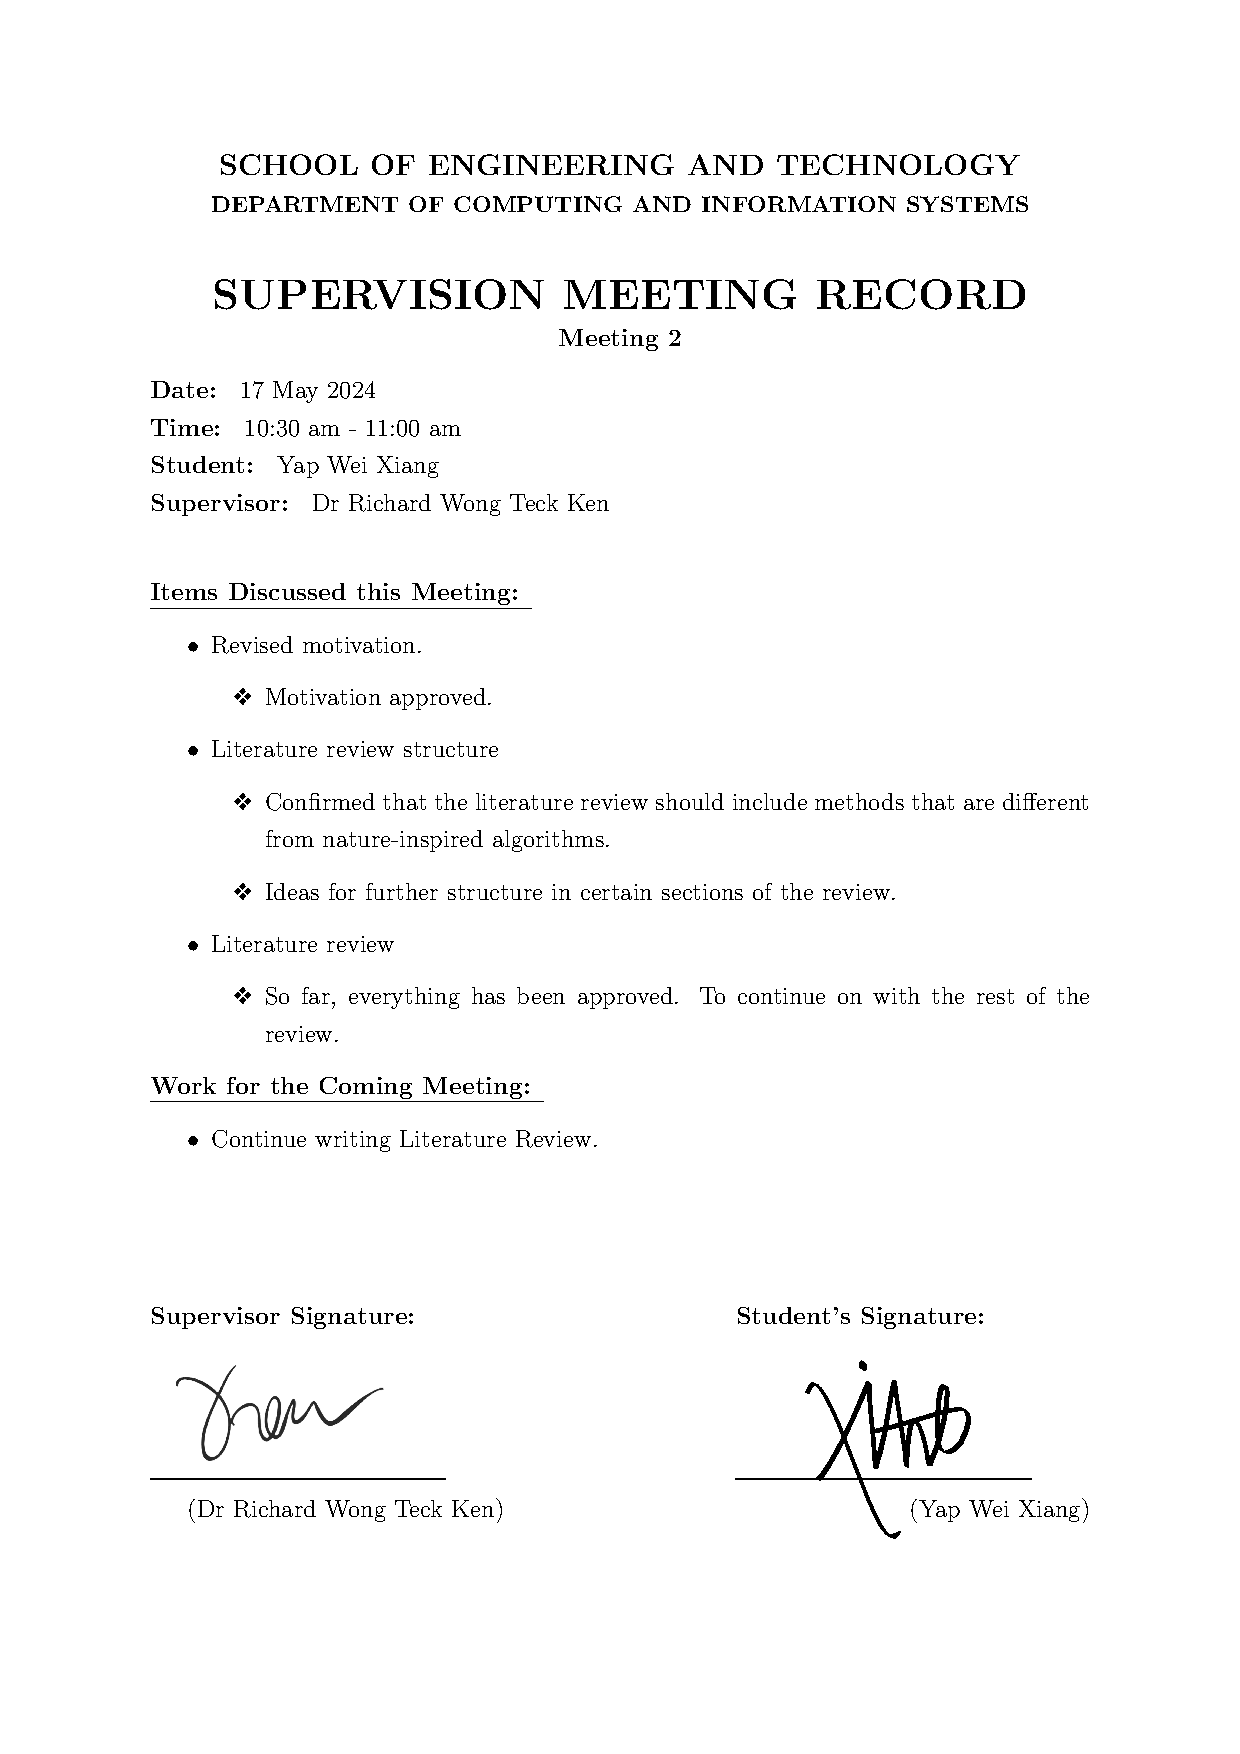
\includepdf[addtotoc={1, section, 1, Meeting 2, meeting2}, pagecommand={\thispagestyle{plain}}]{./meeting-records/signed/meeting-2}
		
		
\includepdf[addtotoc={1, section, 1, Meeting 3, meeting3}, pagecommand={\thispagestyle{plain}}]{./meeting-records/signed/meeting-3}
		
\end{document}